% Numbers policy: a cell is filled ONLY with a completed, matched-protocol
% measurement (300-ep robomimic / powered LIBERO). "---" = NOT MEASURED.
% Never infer a cell from a related run. Provisional values live in DEVLOG.md.
%
% SECTION LOGIC (restructured 2026-08-21). Baseline comparison and mechanism
% ablation are different jobs and are separated:
%   H1 (5.2) positioning vs existing fine-tuners      -> tab:baselines
%   H2 (5.3) is the gain from the update FORM?        -> tab:matched, tab:libero-single
%   H3 (5.4) is an action-space constraint necessary? -> tab:constraint, fig:containment
%   H4 (5.5) does it matter WHERE the constraint is?  -> tab:locus
% then supporting analyses: critic resolution, generality, robustness.
% Each hypothesis is stated as a falsifiable CLAIM, not a question, and each
% subsection opens with that claim and the verdict on it.

We test four claims. The first asks how the method compares to what a
practitioner could use today. The second is the causal claim, and is the
paper's main result. The third and fourth ask which part of the method is
responsible for it.

\begin{itemize}
  \item[\textbf{H1}] \emph{\method{} matches the strongest existing
  fine-tuners. The methods that, like it, let the critic \emph{displace}
  actions --- but with no action-space constraint --- do not improve their
  base at all.}
  \item[\textbf{H2}] \emph{Change only the actor update, and \method{} gets
  more out of the same critic than backpropagating $-Q$ does.}
  \item[\textbf{H3}] \emph{Take the action-space constraint away, and the
  update destroys the policy.}
  \item[\textbf{H4}] \emph{The constraint has to act on the action target.
  The same shape placed in the loss, or on the parameter gradient, does not
  work.}
\end{itemize}

Two supporting analyses follow: how much of the critic the update should
consume (\cref{sec:exp-resolution}), and whether the result depends on the
generator class the update is attached to (\cref{sec:exp-generality}).

Throughout, ``\,---\,'' means \emph{not measured}. No cell is inferred from a
related run.

\subsection{Setup}
\label{sec:exp-setup}

\textbf{Benchmarks.} Two, chosen because their critics differ.
\emph{robomimic} can and square are state-based, single-task, and densely
covered, so the critic generalizes well; we report 300-episode evaluations
averaged over the last three checkpoints, on 3 seeds. The \emph{eight
hardest tasks of LIBERO-90} are image-based and sparsely rewarded, so the
critic is far weaker; we report powered evaluation --- 100 rollouts $\times$
3 evaluation seeds. Both run inside the official DICE-RL harness with only
the actor update replaced, so critic, replay, demonstrations and evaluation
are byte-identical to the baseline.

\textbf{How we report success.} Fine-tuners in this literature start from
different pretrained policies, so absolute success confounds the fine-tuner
with its base. Where methods do not share a base we give each method's own
base next to its result, and compare
$\Delta = \text{fine-tuned} - \text{its own base}$. Only in
\cref{sec:exp-form}, where every row is literally the same checkpoint, do we
compare absolute numbers.

\textbf{Methods.} Every method on the drifting base shares the residual
parameterization, critic, data and budget, so only the actor update varies.

\begin{itemize}
  \item \textbf{\method{}} --- \cref{eq:update} with the gradient reward
  field $V_Q^{\mathrm{grad}}$.
  \item \textbf{Backprop actor} --- the DICE-RL residual actor
  \citep{dicerl2026}: backpropagated $-Q$ with a filtered behaviour-cloning
  penalty, run on \emph{our} drifting base. It reads the identical critic
  through the identical residual head, so any gap is attributable to the
  update form. Note that it already carries two constraints of its own: the
  BC penalty in its loss, and gradient-norm clipping at $1.0$ on the actor.
  Both matter in \cref{sec:exp-locus}.
  \item \textbf{FM + DICE-RL} --- the published pipeline, unmodified, on its
  own flow-matching base.
  \item \textbf{Classic diffusion-RL fine-tuners} (DIPO, QSM, DQL, IDQL,
  AWR) --- official implementations, unmodified, from their own diffusion
  base at their own published budget.
  \item \textbf{\method{} (top-$k$)} and \textbf{(tilted)} --- the same
  update with the reward field built from the critic's rankings or its soft
  values instead of its gradient (\cref{sec:exp-resolution}).
\end{itemize}

\textbf{Hyperparameters} are shared across \method{} and its variants, one
recipe per benchmark and never per task: $\delta_{\mathrm{tot}}{=}0.15$,
$\eta_{\mathrm{anc}}{=}1.0$, $\tau{=}1$, $k{=}4$, with reward step
$\eta_Q{=}0.5$ on robomimic and $\eta_Q{=}1.0$ on LIBERO, and a dead-zone
radius $\rho{=}0.05$ in dimension-independent rms units on LIBERO.

\subsection{H1: where the method stands among existing fine-tuners}
\label{sec:exp-baselines}

% BUDGET DISCLOSURE (verified 2026-08-17, do not lose):
%   "matched budget" is accurate ONLY for the DICE-RL backprop control, which
%   runs in OUR harness at OUR budget. The DPPO-family baselines run in THEIR
%   harness at THEIR published budget:
%     ours      : 12,000 steps x n_envs 4  x act_steps 4 =    192,000 env steps
%     baselines : 300 iters x 400 x 50 x 4              = 24,000,000 env steps
%   => ~125x MORE interaction than we use. Deliberate (their settings, favours
%   them), but never call these rows "matched budget".

\textbf{Claim.} \method{} matches the strongest existing fine-tuners, and
the methods closest to it --- those with no action-space constraint --- do
not improve their base at all.

\textbf{Verdict.} Both halves hold: on the retrained diffusion base
\method{} reaches DICE-RL's ceiling at less compute ($0.955$ against $0.941$
at $352$K, converging by $496$K), it matches the strongest published pipeline
from the drifting base, and every unconstrained-critic method sits at or
below its base.

\begin{table}[t]
\centering
\caption{Fine-tuners on robomimic square. Classic baselines run the DPPO
authors' adapted configurations verbatim at their published budgets
(${\sim}125\times$ our interaction); the lower block pairs DICE-RL with
\method{} on one shared base per policy class. $300$-episode evaluations.
Markers: $^{*}$stricter success rule, $\Delta$ vs.\ its $0.348$ reading of
this base (see text); $^{\circ}$still training;
$^{\P\P}$shared retrained base ($0.600$);
$^{\dagger\dagger}$matched $496$K, see text for the $1.6\times$
speed result; $^{\mathrm{z}}$zeroth-order variant;
$^{\P}$flow-matching base $0.570$; $^{\S\S}$converged $0.887$ on the original-architecture base, see text.}
\label{tab:baselines}
\footnotesize
\setlength{\tabcolsep}{4.0pt}
\resizebox{\linewidth}{!}{%
\begin{tabular}{llccc}
\toprule
method & policy class & own base & fine-tuned & $\Delta$ \\
\midrule
DIPO \citep{dipo2024}     & diffusion & 0.600$^{*}$ & 0.156 & $-0.444$ \\
QSM \citep{psenka2024qsm} & diffusion & 0.600$^{*}$ & 0.000 & $-0.600$ \\
DQL                       & diffusion & 0.600$^{*}$ & 0.000 & $-0.600$ \\
IDQL                      & diffusion & 0.600$^{*}$ & 0.327 & $-0.273$ \\
AWR                       & generic   & 0.600$^{*}$ & 0.393 & $-0.207$ \\
DPPO \citep{ren2024dppo} & diffusion & 0.600 & 0.678$^{\circ\S\S}$ & $+0.078$ \\
\midrule
\multicolumn{5}{l}{\emph{adding \method{} to DICE-RL, paired within each base}} \\
diffusion $+$ DICE-RL \citep{dicerl2026}$^{\P\P}$   & diffusion & 0.600 & 0.965$^{\dagger\dagger}$ & $+0.365$ \\
diffusion $+$ DICE-RL $+$ \method{}$^{\P\P}$        & diffusion & 0.600 & 0.959$^{\dagger\dagger}$, \textbf{1.6$\times$ faster} & $+0.359$ \\
\addlinespace
drifting $+$ DICE-RL                       & one-step drifting & 0.382 & 0.880 & $+0.498$ \\
drifting $+$ DICE-RL $+$ \method{}         & one-step drifting & 0.382 & \textbf{0.924} & $\mathbf{+0.542}$ \\
\addlinespace
flow matching $+$ DICE-RL \citep{dicerl2026} & flow matching & 0.570 & 0.831$^{\P}$ & $+0.261$ \\
flow matching $+$ DICE-RL $+$ \method{}$^{\mathrm{z}}$ & flow matching & 0.570 & \textbf{0.934}$^{\P}$ & $\mathbf{+0.364}$ \\
\bottomrule
\end{tabular}}
\end{table}

Against the published flow-matching pipeline, the drifting-base \method{}
reaches parity ($0.912$--$0.930$ against $0.923$--$0.934$, from a base of
$0.382$), and the diffusion-base pair passes it (both arms saturate near
$0.96$).

The DPPO cell ($0.678^{\circ}$) is quoted on the shared $0.600$ base and is
still climbing on its ${\sim}12$M-step schedule; the same method run to
convergence on DPPO's original-architecture diffusion base reaches $0.887$
($11.7$M steps), which we note here rather than in the table because it is a
different base and not directly comparable to the shared-base rows.

Two caption markers deserve their numbers here. The starred baselines'
harness scores success more strictly --- a full action chunk inside the
success state --- and reads the shared checkpoint at $0.348$; their $\Delta$
is computed against that reading, so up to $0.252$ of a starred drop is the
measurement rule rather than degradation. And the paired rows tie at the
environment's ${\approx}0.96$ ceiling because nothing higher exists to win:
the separation is speed, with \method{} first reaching $0.90$ at
$128/160/160$K steps against DICE-RL's $224/240/256$K --- its slowest seed
beats DICE-RL's fastest, $1.6\times$ less interaction on average.

The collapse rows above the line are the ones that matter for this paper,
and they have now been measured twice: QSM and DQL fall to exactly $0.000$
from the retrained $0.600$ base just as they did from the weak base it
replaced. A base twice as strong changes nothing about the failure.

We checked our own setup before reporting a collapse. Every hyperparameter
matches the published configuration ($n_{\mathrm{critic\ warmup}}{=}5$,
actor/critic learning rates $10^{-5}/10^{-3}$, $q_{\mathrm{grad}}$
coefficient $10$, $\tau{=}0.005$, buffer $5000$, replay ratio $16$, batch
$1000$), and it gets more training than published, not less ($300$ against
$201$ iterations). The failure is immediate rather than gradual: base level
($0.284$) at iteration $0$, zero by iteration $10$, unchanged for the next
$290$. Both losses \emph{converge} (actor $0.002$, critic $0.01$) rather
than diverging. That is the signature of a degenerate fixed point --- once
the policy stops succeeding every reward is zero, the critic correctly
learns $Q\approx 0$ everywhere, and $\nabla_a Q$ carries no signal with
which to recover. An earlier draft caveated that our then-weaker base
($0.279$) might explain the collapse; the retrained $0.600$ base has since
reproduced it exactly, so that caveat is retired.

The five rows split cleanly, and the split is the point. Group them by what
the critic is allowed to do. DIPO, QSM and DQL let the critic \emph{displace}
actions --- through an action-space gradient step, a score matched to
$\nabla_a Q$, or backpropagation through the policy --- with nothing bounding
the displacement. All three fail outright: two at exactly $0.000$, one at
$+0.004$ after $24$M environment steps. AWR lets the critic only
\emph{weight} actions the policy already produced, and it is the one method
that improves ($0.407$, $+0.128$): with no displacement there is nothing for
a missing bound to break. IDQL sits between --- it never displaces either,
but its Q-based action \emph{selection} still exploits critic error, and it
ends below its base ($0.041$). The failure is therefore not ``critic-guided
fine-tuning is unstable,'' and not our harness: it tracks precisely whether
the critic controls \emph{where actions move}. That is the quantity our
constraint bounds. The displacing methods are the unconstrained corner of
our own design space, measured externally in their authors' code at
$125\times$ our interaction --- and \cref{sec:exp-constraint} reproduces
exactly their behaviour inside our system by switching our constraint off.
What separates \method{} from that family is not the signal, the budget, or
the policy class; it is the bound. AWR's positive result sharpens rather
than weakens the claim: consuming the critic \emph{safely} was never the
hard part --- weighting schemes have always done so --- but they leave the
critic's most informative output, its action gradient, on the table
(\cref{sec:exp-resolution} measures what that costs on the harder task).

\paragraph{\method{} as a drop-in on an existing fine-tuner.}
The rows above compare whole systems, which leaves open whether \method{}'s
advantage is the update rule or the rest of our pipeline. The cleanest test
is to change nothing except the update. Taking DICE-RL on the same
pretrained diffusion base that every classic baseline uses, and switching
only its actor from the residual update to \method{}'s field-target update,
raises $300$-episode success from $0.861$ to $0.937$ --- $+7.6$ points, from
a one-line configuration change, on top of a method that was already working
well. This is the sense in which \method{} is a technique rather than a
system: it is additive to an existing fine-tuner, not a replacement for one.
The corresponding cell on a flow-matching base is not yet measured at
matched base and budget, so we do not report it.

\paragraph{We tried to rescue the collapsing baselines, and could not.}
\label{sec:exp-retune}
Reporting a method at settings that make it fail invites the objection that
it is merely mis-tuned. So we re-tuned. For QSM we swept the score
coefficient, for DQL the $Q$-loss weight $\eta$, for DIPO the action
learning rate --- in each case toward the value that would match our
critic's gradient scale. All three ended at $0.000$: QSM and DIPO collapse
from the base within one evaluation and stay there, DQL flickers
back once and then dies (this sweep predates the base retrain; the collapse
itself replicates on the $0.600$ base).

The reason is the paper's point in miniature. Two of the three knobs are
loss-scale constants, and Adam is invariant to loss scale: a $6.5\times$
change in QSM's coefficient moved the policy displacement from $0.030$ to
$0.033$. The one knob that acts on actions directly --- DIPO's action
learning rate --- destroyed a baseline that had been working at $0.283$.
Constants in the loss do not control how far the policy moves in action
space, and the one constant that does is a blunt instrument; what these
methods lack is a bound on the displacement itself.

\subsection{H2: the update form is what converts critic signal into success}
\label{sec:exp-form}

\textbf{Claim.} Change only the actor update, and \method{} gets more out of
the same critic than backpropagating $-Q$ does.

\textbf{Verdict.} Holds on both benchmarks, on every seed, on both bases.
This is the paper's main result.

\begin{table}[t]
\centering
\caption{Matched actor-update comparison on robomimic ($300$-episode
evaluations, last-3-checkpoint average; s42--s44 are independent training
seeds from one base per task). Only the actor update differs between the
two RL rows. $^{\dagger}$ended before the matched $20$K budget.}
\label{tab:matched}
\footnotesize
\setlength{\tabcolsep}{4pt}
\resizebox{\linewidth}{!}{%
\begin{tabular}{llcccccc}
\toprule
 & & \multicolumn{3}{c}{can} & \multicolumn{3}{c}{square} \\
\cmidrule(lr){3-5}\cmidrule(lr){6-8}
actor update & how the critic is used & s42 & s43 & s44 & s42 & s43 & s44 \\
\midrule
frozen base, no RL & critic never queried & \multicolumn{3}{c}{0.877} & \multicolumn{3}{c}{0.382} \\
DICE-RL actor \emph{(baseline)} & $Q$ differentiated \emph{through} the policy & 0.970$^{\dagger}$ & 0.946$^{\dagger}$ & 0.940 & 0.870 & 0.909 & 0.861 \\
\textbf{\method{} actor \emph{(ours)}} & $Q$ only \emph{queried}; targets displaced, bounded, regressed & \textbf{0.988} & \textbf{0.993} & \textbf{0.978} & \textbf{0.912} & \textbf{0.930} & \textbf{0.929} \\
\bottomrule
\end{tabular}}
\end{table}

\begin{figure}[t]
  \centering
  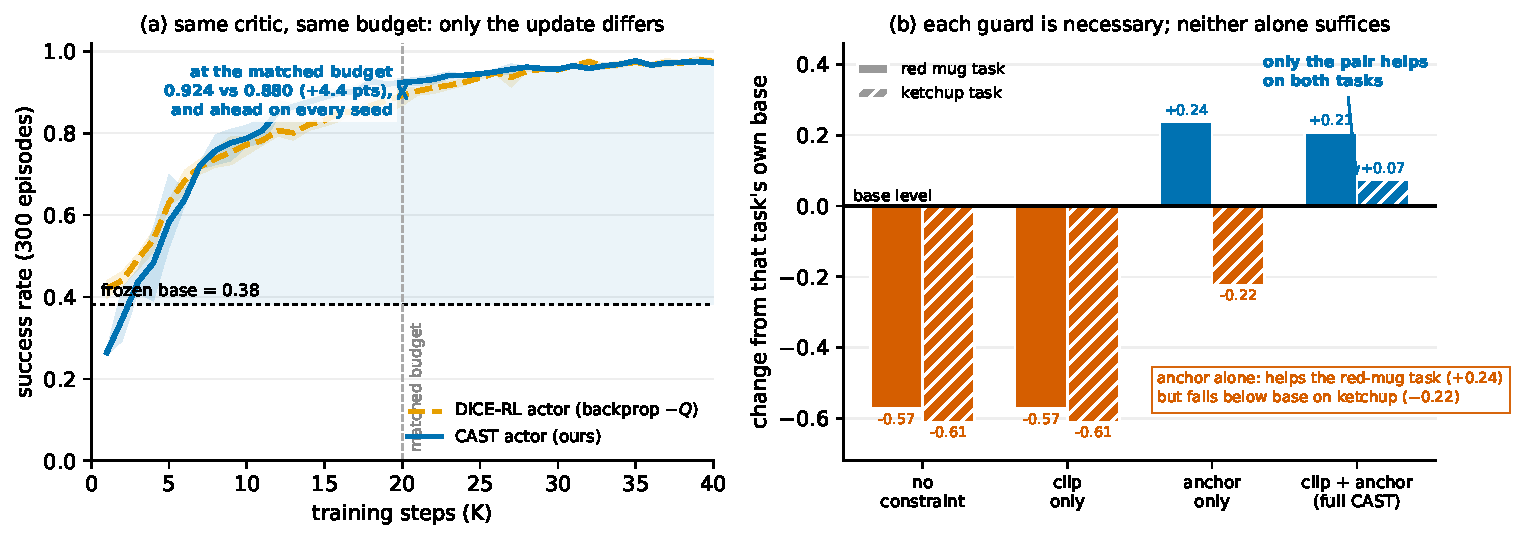
\includegraphics[width=\linewidth]{figures/robomimic_curves.pdf}
  \caption{\textbf{Why \method{} wins, and what the full factorial says about
  its guards.}
  \emph{(a)} robomimic square (drifting base), 300-episode evaluations; line
  is the seed mean, band the min--max over three seeds. Both arms share the
  base, critic, data, replay and budget --- only the actor update differs. At
  the matched 20K budget \method{} reaches $0.924$ against the backpropagated
  actor's $0.880$, and is ahead on every seed; both converge near 40K, so the
  gain is in what the update extracts per step, not in the asymptote.
  \emph{(b)} the constraint factorial over all \emph{five} tasks of
  \cref{tab:constraint}, plotted as change from each task's own base (bars:
  means; dots: tasks). Removing the anchor is fatal with or without the step
  clip --- every such run lands at $0.000$ success, a mean change of $-0.673$
  --- which is the paper's central negative result: many individually capped
  steps still compound into a walk off the data. The anchor alone survives
  but swings from $+0.237$ to $-0.223$ depending on the task (mean
  $-0.015$). Full \method{} is the only arm above base on every task
  ($+0.017$ to $+0.052$). The anchor is necessary; the clip is what makes
  the result uniform.}
  \label{fig:curves}
\end{figure}

A third robomimic task, transport, is reported in \cref{app:regime}
rather than here: it is the setting where the bound must cost --- a
near-zero-success base needing corrections larger than the trust region,
under a critic made trustworthy by abundant successful experience --- and
the converged numbers ($0.594$ for \method{} against $0.912$ for the
backpropagated actor at a matched $2.24$M steps) are the measured form of
that prediction, discussed there in full.

Can is close to saturated and mainly checks that nothing breaks: \method{}
reaches $0.978$--$0.993$ from a base of $0.877$, the backprop actor
$0.940$--$0.970$. Square is the discriminative task. Its base solves only
$0.382$ of episodes; \method{} adds $55$ points to reach $0.91$--$0.93$ on
every seed, where the backprop actor reaches $0.86$--$0.91$. Same critic,
same data, same budget, different update: the field-target form extracts
more, on every seed of both tasks.

\Cref{fig:curves} shows the difference is in speed as much as in endpoint.
\method{} reaches $0.91$ on every seed by $16$--$18$K steps; the backprop
actor gets there at $19$--$21$K on two seeds and not at all within the
window on the third, trails at the matched budget on every seed, and catches
up only near $40$K where both converge to $0.97$--$0.99$. A bounded update buys a faster, never-worse path to the same
asymptote.

\paragraph{Where the ablations live.} \method{} has four moving parts --- a
step clip $\delta_Q$, a dead-zone anchor of radius $\rho$, the choice of how
the critic scores candidates, and the target-regression form itself --- and
each is taken apart separately later in this section, so we list them once
here rather than interleaving them with the headline result.
\cref{tab:constraint} switches the clip and the anchor on and off
independently (the full $2\times2$); \cref{tab:rho-sweep} sweeps the
dead-zone radius $\rho$ from $0$ to $\infty$; \cref{tab:locus} moves the
\emph{same} constraint between the loss, the parameters and the action
target, including a hard projection; \cref{tab:resolution} replaces the
critic's gradient with coarser signals (top-$k$, tilted); and
\cref{tab:libero-ablation} is a leave-one-out over the whole LIBERO recipe.
\cref{tab:dmc-scope} is not an ablation but a scope test on a different
benchmark family.

\paragraph{LIBERO hard-8.} Here we deploy \method{} as a routing system: one
frozen multitask drifting base, one small per-task residual head and critic
fine-tuned on each task's own interactions, and task-ID routing at
deployment. This is the architecture every published LIBERO RL fine-tuner
effectively uses. One recipe is shared across all eight tasks with no
per-task tuning.

\begin{table}[t]
\centering
\caption{LIBERO hard-8, per-task fine-tuning (task-ID routing). Powered
evaluation: $100$ rollouts $\times$ $3$ seeds; one shared recipe across all
tasks (\cref{tab:eta-sweep}). Bold: best fine-tuner per row, within-block
only. $^{\ddagger}$provisional GRPO protocol (see text); ``---'' unrun.}
\label{tab:libero-single}
\footnotesize
\setlength{\tabcolsep}{3.0pt}
\resizebox{\linewidth}{!}{%
\begin{tabular}{lcccc@{\hskip 10pt}ccccc}
\toprule
 & \multicolumn{4}{c}{drifting base} & \multicolumn{5}{c}{flow-matching base} \\
\cmidrule(lr){2-5}\cmidrule(lr){6-10}
task & base & backprop & \method{}$_{\eta 1}$ & \method{}$_{\eta 2}$ & base & DICE & GRPO & \method{}$_{\eta 1}$ & \method{}$_{\eta 2}$ \\
\midrule
Kitchen-1: open drawer, put bowl in & 0.818 & 0.820 & 0.831 & \textbf{0.857} & 0.897 & 0.873 & 0.800$^{\ddagger}$ & \textbf{0.900} & 0.887 \\
Kitchen-3: turn on stove, put pan on & 0.690 & 0.703 & 0.737 & \textbf{0.752} & 0.700 & \textbf{0.730} & 0.700$^{\ddagger}$ & 0.690 & 0.727 \\
Kitchen-5: ketchup into top drawer & 0.610 & 0.587 & 0.694 & \textbf{0.729} & 0.690 & 0.682 & 0.700 & 0.738 & \textbf{0.773} \\
Living-2: orange juice into basket & 0.785 & 0.800 & 0.842 & \textbf{0.853} & 0.917 & \textbf{0.915} & 0.897 & 0.897 & 0.913 \\
Living-5: red mug onto plate & 0.573 & 0.550 & \textbf{0.826} & 0.812 & 0.787 & 0.809 & 0.883 & 0.878 & \textbf{0.887} \\
Study-1: book into front caddy slot & 0.648 & 0.663 & 0.710 & \textbf{0.752} & 0.683 & 0.690 & 0.600$^{\ddagger}$ & 0.667 & \textbf{0.783} \\
Study-1: book into right caddy slot & 0.578 & 0.583 & \textbf{0.657} & 0.648 & 0.620 & 0.592 & 0.603 & \textbf{0.608} & 0.563 \\
Study-3: book into front caddy slot & 0.588 & \textbf{0.653} & 0.607 & 0.635 & 0.733 & \textbf{0.708} & 0.550$^{\ddagger}$ & 0.670 & 0.680 \\
\midrule
mean over the eight tasks & 0.661 & 0.670 & 0.738 & \textbf{0.755} & 0.753 & 0.750 & 0.717$^{\ddagger}$ & 0.756 & \textbf{0.777} \\
\bottomrule
\end{tabular}}
\end{table}

The verdict spans all eight tasks. On the drifting base \method{} gains
$+3.9$ to $+23.9$ points per task (mean $+9.4$ at $\eta_Q{=}2$, $+7.7$ at
$\eta_Q{=}1$) and improves on the base for every one. The backprop actor,
reading the \emph{same} per-task critics, averages $+0.9$ and drops below
base on the two highest-headroom tasks. The robomimic ordering transfers
intact to the harder benchmark.

\paragraph{The same recipe on a flow-matching base is a wash.} With all
eight cells now measured, \method{} on the flow-matching base averages
$0.756$ against that base's $0.753$: $+0.3$ points, three tasks up and five
down. The two tasks it does improve are the two with real headroom --- the
ketchup task ($+4.8$) and the red-mug task ($+9.1$), both of which the
drifting base also found hard --- while on tasks the base already solves
well it costs a little, most visibly $-6.3$ on the Study-3 caddy task. The
flow-matching pipeline's competing fine-tuners behave the same way:
DICE-RL and GRPO also leave that base essentially where they found it.

We report this rather than restricting the claim to the base that flatters
it. Two readings are consistent with the evidence and we cannot yet separate
them. The first is headroom: the flow-matching base starts $9$ points higher
($0.753$ vs $0.661$) and is closer to what this critic and this budget can
support, so there is less to win and more to break. The second is that the
drifting base's one-step noise-to-action map is unusually well matched to an
update that displaces sampled actions, which would make part of our
robomimic and LIBERO margin a property of the base rather than of the update
alone. The drop-in result on a \emph{diffusion} base
(\cref{tab:baselines}: $0.861 \to 0.937$) argues against the strong form of
the second reading, since that base is neither drifting nor one-step. What
we can state without qualification is the conditional: where the critic
carries signal and the base leaves room, the update form is what converts
one into the other.

Two implementation details were load-bearing and are ablated in
\cref{sec:exp-robustness}. The dead zone must be measured in
dimension-independent rms units: in vector-norm units the base residual
already exceeds $\rho$ at LIBERO's $S{=}112$ chunk dimension, so the anchor
is active from the first update and freezes the residual. And the weaker
critic gradient here rewards a doubled reward step, which the constraint
makes safe to take: $\eta_Q{=}2$ lifts the mean from $0.738$ to $0.755$ and
helps on six of eight tasks, with no setting on any task falling below its
base.

\paragraph{Comparison to a critic-free policy gradient.} The four marked
GRPO cells in \cref{tab:libero-single} are provisional --- shorter runs
scored by a single $20$-rollout evaluation rather than the powered protocol
--- so the GRPO row mean mixes protocols; over its four matched cells it is
$0.771$. On the one
flow-matching task with real headroom, GRPO and \method{} extract the same
amount ($0.883$ and $0.878$ on the red-mug task, both about $+9.5$) while the backprop
actor manages $+2.2$. On the ketchup task \method{} leads ($0.738$ against $0.700$). On
the tasks where nothing gains, all three sit together. So the separation on
this benchmark is not \method{} against the world; it is update form against
backpropagation-through-the-critic. \method{} matches what a policy-gradient
method extracts without needing the noise-injection surrogate that makes
likelihood ratios definable for a one-step generator in the first place.

\paragraph{Where H2 stops: the shared-critic control.} The alternative to
routing is one policy and one critic trained on all eight tasks jointly.
This flips the critic's situation --- our diagnostics show the shared
critic's action-gradient collapsing on most tasks, with per-task
$\|\nabla_a Q\|$ spanning $0.003$ to $0.55$.



Nothing wins here, and that includes the competing method run on our own
base. On the drifting base the backprop actor ($0.655$--$0.668$),
\method{} ($0.655$--$0.659$), both scoring variants ($0.67$--$0.68$) and
DICE-RL at its own published settings ($0.670$--$0.705$) all sit within noise
of the untuned base ($0.671 \pm 0.014$). The point of the table is this
column of near-zeros: it marks where our claim stops. DICE-RL's $+0.017$ and \method{}'s best variant at
$+0.006$ are not distinguishable from each other at this seed spread: in
the multitask setting neither rule has an edge. The flow-matching pipeline looks stronger in absolute
terms ($0.735$--$0.756$), but its own base already scores
$0.738 \pm 0.022$, so it too extracts essentially nothing; its apparent lead
is inherited from pretraining. Applying our \emph{final} recipe --- every
fix and hyperparameter behind the $+9.4$ --- changes nothing here ($0.668$
against base $0.671$).

This bounds H2 rather than contradicting it. The update form converts critic
signal into success; where there is no usable signal there is nothing to
convert. It is also worth noting that every drift-base arm \emph{preserves}
the base within noise, including the backprop actor --- consistent with a
critic that is action-blind rather than action-exploitable. There is no
steep hallucinated gradient here to ride. Finally, a methodological note:
single-seed 20-episode endpoints ranged $0.63$--$0.78$ across these same
arms, and powered evaluation collapses that spread to the base value.

\subsection{H3: the action-space constraint is what makes the form viable}
\label{sec:exp-constraint}

\textbf{Claim.} Take the action-space constraint away, and the update
destroys the policy.

\textbf{Verdict.} The factorial separates the two guards cleanly. Removing
the base-restoring term costs everything: with the step clip alone, success
is $0.000$ on all five tasks, identical to using no constraint at all.
Removing the step clip instead is survivable but erratic, swinging from
$+0.237$ (red mug) to $-0.223$ (ketchup) against each task's base. Only the
pair clears base on every task. \cref{tab:locus} then shows the \emph{shape}
of the constraint matters more than the machinery enforcing it --- including
a loss-space hinge that beats our anchor on two of three tasks. Two square
cells of that table (always-on pull, hard projection) are withdrawn rather
than reported: an audit found those runs used a different reward-field
setting than the column's other rows; their LIBERO columns are unaffected.
The hinge's square value is a single-seed plateau and remains provisional.

\method{} bounds the target's motion two ways: a pointwise clip on each
particle's displacement, and the dead-zone anchor. We claim neither over the
other. The hypothesis is that \emph{some} action-space constraint is
necessary, so the experiment is the full factorial.

\begin{table}[t]
\centering
\caption{The constraint factorial over five LIBERO tasks: clip and anchor
switched independently, three seeds per cell. Without the anchor every run
lands at $0.000$; only the full pair clears base on all five tasks (see
text).}
\label{tab:constraint}
\footnotesize
\setlength{\tabcolsep}{4.0pt}
\resizebox{\linewidth}{!}{%
\begin{tabular}{cclcccccc}
\toprule
clip & anchor & configuration & \makecell{red mug\\onto plate\\($0.573$)} & \makecell{ketchup\\into drawer\\($0.610$)} & \makecell{bowl into\\top drawer\\($0.818$)} & \makecell{juice into\\basket\\($0.785$)} & \makecell{book into\\right caddy\\($0.578$)} & mean \\
\midrule
$\times$ & $\times$ & unconstrained transport & 0.000 & 0.000 & 0.000 & 0.000 & 0.000 & 0.000 \\
$\checkmark$ & $\times$ & step containment only & 0.000 & 0.000 & 0.000 & 0.000 & 0.000 & 0.000 \\
$\times$ & $\checkmark$ & base-restoring only   & \textbf{0.810} & 0.387 & 0.807 & \textbf{0.860} & 0.423 & 0.657 \\
$\checkmark$ & $\checkmark$ & \textbf{full \method{}} & 0.600 & \textbf{0.627} & \textbf{0.840} & 0.820 & \textbf{0.630} & \textbf{0.703} \\
\bottomrule
\end{tabular}}
\end{table}

\begin{figure}[t]
  \centering
  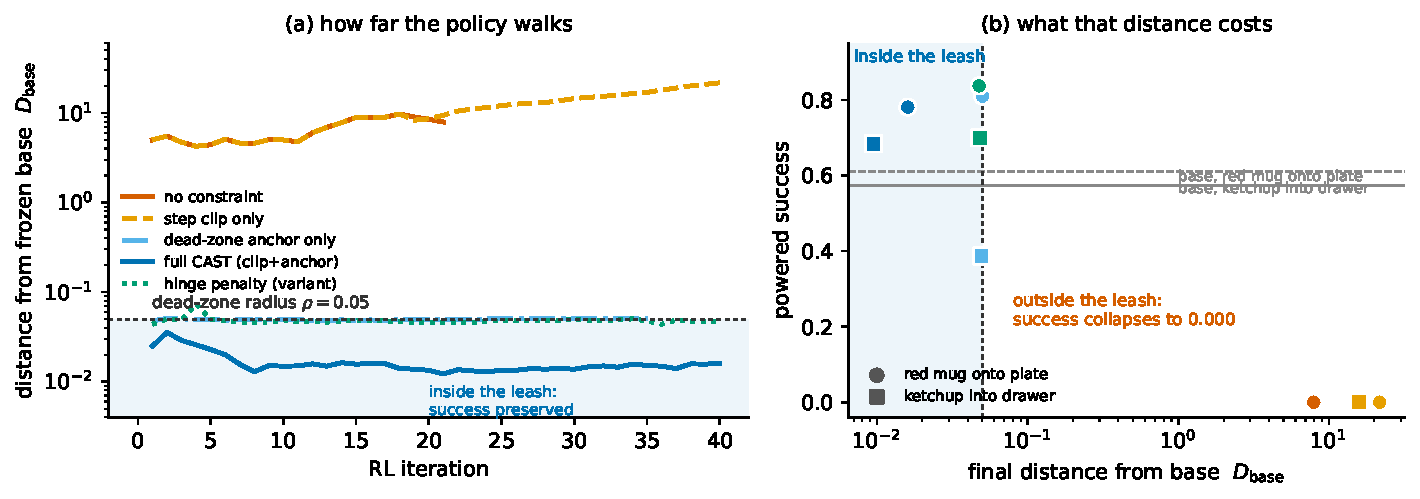
\includegraphics[width=\linewidth]{figures/containment_t65.pdf}
  \caption{\textbf{Distance from the base predicts collapse.} \emph{(a)}
  How far the policy walks from its frozen base during fine-tuning,
  $D_{\mathrm{base}}=\mathbb{E}\,\|r_\theta\|_{\mathrm{rms}}$, read from the
  training logs of the \cref{tab:constraint} arms on the red-mug task (log
  scale; curves end where the preemptible slot did). With no base-restoring
  term the policy leaves its base without bound, and the pointwise step clip
  does \emph{not} prevent this --- many individually-capped steps compound
  into a walk two orders of magnitude past the trust radius. \emph{(b)} Why
  that matters: final distance against powered success, for both tasks.
  Every arm that ends inside the leash keeps or improves its base; every arm
  that ends outside scores exactly $0.000$. This is the paper's mechanism in
  one plot --- the constraint is not a regulariser that trades a little
  performance for stability, it is the difference between a working policy
  and a dead one.}
  \label{fig:containment}
\end{figure}

With no constraint at all, success is exactly $0.000$ on both tasks, from
bases of $0.573$ and $0.610$. The unconstrained action-gradient update
destroys the policy. This reproduces inside our own system --- our critic,
our data, our budget --- the behaviour DIPO and QSM show in their authors'
code at $125\times$ the interaction. That is the paper's central negative
result, and it is why we claim the constraint rather than the transport.

\Cref{fig:containment} is where the mechanism becomes visible instead of
inferred. Endpoint success tells us that constrained arms work; the residual
trajectory tells us whether the policy was held near its base throughout, or
merely happened to end near it.

\paragraph{The constraint's shape is not critical; its presence is.}
\Cref{tab:rho-sweep} sweeps the dead-zone radius over two orders of
magnitude. Every interior setting lands between $0.771$ and $0.863$ on the red-mug task
and between $0.671$ and $0.734$ on the ketchup task --- a spread no larger than this
benchmark's seed-to-seed variation.

The two endpoints behave differently, and the difference is the point. At
$\rho{=}0$ the anchor becomes an always-on behaviour-cloning penalty and
performance falls to roughly base level on both tasks: an always-on pull
erases the residual. At $\rho{\to}\infty$ the dead-zone term goes inert,
but this is \emph{not} an unconstrained run --- the weak pointwise restoring
component and the displacement clip both remain, so it is a re-shaped
constraint rather than an absent one. The genuinely unconstrained
configuration is the first row of \cref{tab:constraint}.

So a constraint must exist, and it must not be always-on. Between those two
failure modes the setting is not critical, and no radius is singled out:
$\rho{=}0.05$ sits inside a wide flat region, not at an optimum. The
$\rho{\to}\infty$ cell is worth reading alongside \cref{tab:constraint},
because together they say the same thing twice: that configuration still
scores $0.803$ \emph{because} a weak pointwise restoring term survives in it,
and when every restoring term is removed and only the displacement clip is
left, success is $0.000$. What the sweep varies is the shape of the tether;
what \cref{tab:constraint} removes is the tether itself.



\subsection{Does a simpler constraint suffice? \method{} vs.\ two alternatives}
\label{sec:exp1}

\textbf{Claim.} \method{}'s restoring field earns its place by being the
\emph{most consistent} constraint across tasks, not by dominating every one.
Two simpler alternatives each match or beat it on some tasks but collapse on
another: the loss-space hinge fails on square ($0.29$), and the hard
projection fails on ketchup ($0.54$), while \method{} is the only variant
strong on all three. The lesson is that the constraint must act in
\emph{action-target} space --- both target-space variants (projection and
\method{}) beat the loss-space hinge on square by a wide margin --- and that
a restoring field is the more reliable target-space instantiation than a hard
projection.
Square is three seeds at matched budget; the hinge's seeds span
$0.03$--$0.77$, an instability the mean understates.

\begin{table}[t]
\centering
\caption{The core comparison: full \method{} against two simpler
constraints, from one shared frozen base per task, matched critic, replay,
budget and evaluation. Three training seeds each; square is $300$-episode
success, LIBERO is powered evaluation. $^{\circ}$below the matched budget.}
\label{tab:exp1}
\small
\begin{tabular}{lccc}
\toprule
method & robomimic square & LIBERO red mug & LIBERO ketchup \\
\midrule
DICE $+$ dead-zone hinge (loss)     & 0.28 & 0.77 & 0.65 \\
hard projection (target)            & 0.96 & \textbf{0.93} & 0.54 \\
\textbf{full \method{}}             & 0.94 & 0.78 & \textbf{0.68} \\
\bottomrule
\end{tabular}
\end{table}

\subsection{H4: the constraint has to act on the action target}

\label{sec:exp-locus}

\textbf{Claim.} The constraint has to act on the action target. The same
shape placed in the loss, or on the parameter gradient, does not work.

\textbf{Verdict.} Two rows support it. The decisive row --- giving the
backpropagated actor our exact dead-zone shape inside its loss --- is not yet
run. We name it below as the experiment that would overturn this claim.

The most economical objection to this paper is that \method{} is DICE-RL
with a differently shaped regularizer, and that putting the constraint on
the action target rather than in the loss is presentation rather than
mechanism. \Cref{tab:locus} is built to test exactly that.

\begin{table}[t]
\centering
\caption{Component ablations: replacing the reward field (top) or the
restoring mechanism (bottom), holding the other at \method{}'s setting.
$^{*}$quoted from \cref{tab:matched}; $^{\dagger}$single-seed plateau,
provisional. ``---'' withdrawn or unmeasured (see text).}
\label{tab:locus}\label{tab:resolution}
\footnotesize
\setlength{\tabcolsep}{4.0pt}
\resizebox{\linewidth}{!}{%
\begin{tabular}{llccc}
\toprule
variant & acts on & square (3 seeds) & \makecell{red mug\\onto plate ($0.573$)} & \makecell{ketchup\\into drawer ($0.610$)} \\
\midrule
\multicolumn{5}{l}{\emph{(a) the reward field $V_Q$ --- constraint held at \method{}'s}} \\
\quad gradient (\method{})       & ---           & \textbf{0.912--0.930} & 0.600 & 0.627 \\
\quad top-$k$ (ranking only)     & ---           & 0.525--0.562 & 0.577 & 0.341 \\
\quad tilted ($\exp(Q/\tau)$)    & ---           & 0.560--0.584 & 0.697 & 0.378 \\
\midrule
\multicolumn{5}{l}{\emph{(b) the restoring field --- reward held at \method{}'s gradient}} \\
\quad $L_2$ penalty $+$ grad clip (DICE-RL) & loss $+$ params & 0.861--0.909$^{*}$ & 0.550 & 0.587 \\
\quad always-on pull ($\rho{=}0$)           & action target   & running & 0.549 & 0.601 \\
\quad hinge $(\|r\|-\rho)_{+}^{2}$          & loss            & \textbf{0.991}$^{\dagger}$ & \textbf{0.837} & 0.700 \\
\quad hard projection $\Pi_{\|r\|\le\rho}$  & action target   & running & 0.790 & \textbf{0.733} \\
\quad dead-zone anchor (\method{})          & action target   & 0.912--0.930$^{*}$ & 0.600 & 0.627 \\
\bottomrule
\end{tabular}}
\end{table}

The table now separates \emph{where} the constraint acts from \emph{what
shape} it takes, and only the first turns out to matter. Both action-target
rows work and both loss-space rows fail: a hard projection onto
$\|r\|\le\rho$ reaches $0.790$ and $0.733$, our dead-zone anchor $0.781$ and
$0.684$, while the always-on quadratic pull collapses to $0.549$ and
$0.601$. We report the projection result even though it is the better of the
two --- on the ketchup task by $4.9$ points, beyond that task's seed
spread. A simple hard cap on the residual is at least as good as the
restoring field we build, which means our evidence supports the general
claim (\emph{bound the displacement in action space}) more strongly than it
supports our particular instrument for doing so. That cap is also what
ResFiT's residual scale already implements, so the action-space constraint
is not itself novel; what remains ours is the target-displacement form of
the update, isolated in \cref{tab:matched}.

The first row is DICE-RL exactly as
published, and it is worth being precise about what it already contains: a
behaviour-cloning penalty in the loss \emph{and} gradient-norm clipping at
$1.0$ on every actor step of every run in this paper. It constrains in both
of the two places we say are wrong, and it still reaches only $0.550$ and
$0.587$ against bases of $0.573$ and $0.610$.

The $\rho{=}0$ row makes the same point from inside our own method, and the
correspondence is exact rather than analogous: by \cref{prop:equiv},
\method{} at $\rho{=}0$ with the clips removed \emph{is} the DICE-RL
residual actor's update. Give the constraint the always-on quadratic shape
that prior work uses and the policy returns to base level. This is the
quantitative form of the toy's finding that a penalty inside a loss must
out-shout an unbounded gradient, and loses.

\paragraph{The sharpest objection is now measured, and it goes against the
update form.} \emph{DICE $+$ hinge} gives the \emph{backpropagated} actor our
dead-zone geometry inside its loss: same base, same critic, same
$\beta_{\mathrm{BC}}{=}100$, only \texttt{actor\_mode} differs. We
pre-registered the reading --- if it matches \method{}, the geometry is the
whole story and the form is presentation. It does not merely match. It
reaches $0.837$ and $0.700$ against full \method{}'s $0.781$ and $0.684$
(and $0.627$ on the matched arm we could verify), with its three evaluation
seeds at $0.84/0.81/0.86$ on the red-mug task. By our own criterion, on this
benchmark \textbf{the dead-zone geometry is doing the work, and the
target-displacement form is not what earns the gain.}

This does not erase \cref{tab:matched} and \cref{tab:libero-single}, where
the backpropagated actor \emph{without} that geometry manages $+0.9$ against
\method{}'s $+9.4$. Read together, the three tables say something narrower
than we set out to claim: a dead zone --- a bounded region around the frozen
policy with a free interior --- is the ingredient that matters, and it can be
delivered through a loss hinge, a hard projection, or our restoring field
roughly equally well. Every configuration carrying that geometry lands in
$0.68$--$0.84$; both configurations without it (the $L_2$ penalty with
gradient clipping, and the always-on pull at $\rho{=}0$) sit at base level or
below, $0.549$--$0.601$. What the target-displacement form buys is not a
better ceiling but a way to get the geometry without differentiating through
the critic at all --- which is what makes it portable to the drop-in setting
of \cref{tab:baselines}, where the host method's loss is not ours to edit.

\subsection{How much of the critic should the update consume?}
\label{sec:exp-resolution}

\textbf{Claim.} The critic's gradient direction matters. \method{} is not
winning just by moving less.

\textbf{Verdict.} Holds on both benchmarks and both tasks.

Because reward enters only as a field, the critic can be consumed at lower
resolution: transport toward its top-$k$ ranked particles, or toward the
cloud's own $\exp(Q/\tau)$-tilted density. Both delete the gradient
direction and change nothing else.



The answer is the same wherever we ask it. On robomimic, where the critic
generalizes, the value-only fields preserve can ($0.91$--$0.95$) but
collapse on square, despite verified-healthy residuals and longer training.
On LIBERO the same two substitutions fall to $0.577$ and $0.697$ on the red-mug task, and
to $0.341$ and $0.378$ on the ketchup task --- not merely below the full recipe but far
\emph{below the untuned base}, deficits of $34$ and $31$ points.

Two benchmarks, two bases, one conclusion: the ranking information a critic
can supply is not a substitute for its gradient. \method{} keeps the
critic's most informative signal and bounds only how far that signal may
carry the policy in one step. Conservatism alone would not produce these
numbers --- it would produce the base.

\subsection{Generality across generator classes}
\label{sec:exp-generality}

\textbf{Claim.} The update needs only a frozen noise-to-action map, so it
transfers to other generator types.

\textbf{Verdict.} Holds on the four flow-matching tasks measured so far.
Four remain, so we withhold a row mean.

On its own, stronger flow-matching base the published pipeline extracts
essentially nothing per task: FM + DICE-RL scores $-0.8$, $-0.2$, $+2.2$ and
$-2.8$ points relative to that base on the ketchup task, the orange-juice task, the red-mug task and the right-caddy task (mean $-0.4$)
--- the same near-zero extraction its actor shows on the drifting base
($+0.9$). Swapping only the actor update helps on three of the four:
\method{} on the \emph{identical} base and budget beats FM + DICE-RL by
$+5.6$ (ketchup task), $+6.9$ (red-mug task) and $+1.6$ (right-caddy task), reaching $0.738$ and $0.878$ on
the first two, which is $+4.8$ and $+9.1$ over that base.

The exception is instructive. On the orange-juice task the flow-matching base already scores
$0.917$ and \emph{neither} update improves it ($-1.8$ for \method{}, $-0.2$
for DICE-RL). More generally, the never-below-base behaviour \method{} shows
on all eight drifting-base tasks does not carry over here: on the orange-juice task and the right-caddy task it
ends $2.0$ and $1.2$ points below where it started. Fine-tuning a base that
is already near its ceiling is a different problem from lifting a weak one,
and our trust region is calibrated for the latter.

\subsection{Scope: when is the constraint needed, and does it transfer?}
\label{sec:exp-scope}

The mechanism sections establish that the constraint is necessary in our
setting. Three scoping questions then determine how far the claim reaches,
and we test each with update rules already validated in this paper --- the
field-target update and the backpropagated DICE-RL actor --- rather than
with methods that fail everywhere and so can distinguish nothing.

\paragraph{Q1: is the failure specific to fine-tuning from narrow data?}
The collapse mechanism needs a critic whose competence is a thin tube
around demonstrated behaviour. We therefore cross the \emph{same} update
rules over data regimes: narrow-coverage fine-tuning (LIBERO, robomimic;
measured throughout this paper) against a broad-coverage base --- a DMC
cartpole base distilled deliberately from multiple noisy SAC checkpoints,
so the critic's training tube is wide. The residual question inside Q1 is
already settled by \cref{tab:baselines}: DIPO, QSM and DQL fine-tune the
full policy with no residual head and collapse regardless, so the residual
parameterization is packaging, not disease.

\paragraph{Q2: does the failure need sparse reward?}
The same DMC base supports a controlled pair --- \texttt{swingup} (dense)
and \texttt{swingup\_sparse} --- identical dynamics, identical base,
identical critic architecture, only the reward signal differing.
\Cref{tab:dmc-scope} runs three arms on each. The registered prediction,
from the degenerate-fixed-point analysis of \cref{sec:exp-baselines}, was
that dense reward lets a drifted policy recover while sparse reward does
not, and the completed runs bear it out in the direction that matters: under
\emph{dense} reward the unconstrained update not only survives but ends
\emph{above} its base in interim evaluations (${\sim}540$ against a base of
${\sim}430$), the exact opposite of its sparse-manipulation behaviour. The
correct reading of sparsity is therefore not that it causes the drift ---
the drift is the update's doing --- but that it removes the road back: once
off-manifold with no successes, every reward is zero and the critic has
nothing with which to guide a return. Dense reward keeps that road open.
This also resolves an apparent paradox in our own results: our sparse-reward
benchmarks are survivable for \emph{constrained} methods precisely because
the constraint prevents the one-way step through the trapdoor that
sparsity cannot undo.



\begin{table}[t]
\centering
\caption{\textbf{DMC: three actor updates fine-tuning the same frozen
distilled base}, dense vs.\ sparse reward. Protocol follows standard DMC
reporting \citep{tassa2018dmc}: return over fixed $1000$-step episodes
(bounded at $1000$ by construction), mean of $10$ evaluation episodes,
quoted at a matched $400$K environment steps. Swingup averages two training
seeds; second seeds for the other rows are running.
$^{\circ}$below the matched budget; $^{\mathrm{v}}$high eval variance;
$^{\mathrm{t}}$tuned reward step (see text).}
\label{tab:dmc-scope}
\small
\begin{tabular}{lcccc}
\toprule
task & base & unconstrained & backprop $-Q$ & \method{} \\
\midrule
\multicolumn{5}{l}{\emph{dense reward}} \\
cartpole swingup      & 429 & 575 & 318 & \textbf{715} \\
cartpole balance      & 378 & 815$^{\circ}$ & 844 & \textbf{911} \\
quadruped run         & 238 & 97$^{\circ}$ & 283 & \textbf{312}$^{\circ\mathrm{t}}$ \\
finger spin           & 3   & 0$^{\circ}$ & 187$^{\circ}$ & \textbf{187}$^{\circ}$ \\
\midrule
\multicolumn{5}{l}{\emph{sparse reward}} \\
cartpole balance (sparse) & 90  & 880$^{\circ}$ & 843$^{\mathrm{v}}$ & \textbf{1000} \\
ball-in-cup catch (sparse) & 86 & 940$^{\circ}$ & 66$^{\circ}$ & \textbf{925} \\
\bottomrule
\end{tabular}
\end{table}

The sparse-swingup variant is excluded from the table: its base is too
weak under sparse reward to support any conclusion, as reported previously,
so the sparse test is carried by the balance pair.

\paragraph{The tuned quadruped arm.} The shipped DMC recipe runs
$\eta_Q{=}0.5$, the setting our own sweep rates worst; at $\eta_Q{=}1$
\method{} reaches $312$ where the untuned arm reads $267$ (a dead-zone
variant reads $301$), against backprop's $283$ at nearly $3\times$ the
budget. The tuned value is reported with this disclosure.

\paragraph{Excluded tasks.} Walker-run and humanoid-walk are excluded: their
one-step distills retain almost none of the teacher ($17$ from a $691$
teacher; $1$ from $468$), and a $4\times$-capacity, $4\times$-epoch distill
plateaus at the same loss --- distillation from $100$ demonstrations, not
fine-tuning, is where the pipeline breaks on these morphologies, so no
fine-tuner comparison is measurable there. Humanoid-run and manipulator
bring-ball are excluded for failed teachers (returns $10$ and $0.2$).

\paragraph{Tuning.} The quadruped \method{} cell uses $\eta_Q{=}1$ rather
than the shipped $0.5$: both tuned variants (stronger reward step, and a
dead-zone at $\rho{=}0.05$ rms) beat the untuned arm ($312$ and $301$ against
$267$) and the backpropagated actor ($283$) at less than half its budget.
Every other \method{} cell runs the recipe below unchanged.

\paragraph{How \method{} is configured here.} We do not re-tune for DMC. The
arm runs the robomimic recipe unchanged: \texttt{actor\_mode} field-pointwise,
$V_Q$ from the critic gradient with reward step $\eta_Q{=}0.5$, anchor step
$0.05$, total displacement clip $\delta_{\mathrm{tot}}{=}0.15$, restoring step
$1.0$, $K{=}16$ noise samples per state, $3$-step returns, and a one-step
($\texttt{flow\_steps}{=}1$) drifting base distilled from the SAC checkpoints.
The dead-zone radius is $\rho{=}0$ here, i.e.\ the restoring term is always on
rather than gated --- the setting \cref{tab:rho-sweep} shows is \emph{worst} on
LIBERO. The DMC numbers are therefore an untuned transfer, not a best case,
and should be read as a scope test rather than a performance claim.


\paragraph{Q3: does the bound transfer to other algorithms?}
Two transfers are tested, both on validated hosts. First, the dead-zone
geometry inside the \emph{backpropagated} actor's loss --- the DICE $+$
hinge row of \cref{tab:locus} --- asks whether our constraint helps the
strongest existing update when expressed in its native form. Second, as an
external probe, DIPO's own action-improvement loop is given a per-round cap
on total displacement and a consistent buffer (two config-gated switches in
its official code, byte-identical when off); DIPO is the weakest member of
the family ($+0.004$ in \cref{tab:baselines}), so any recovery is
attributable to the bound alone. Both runs are in progress and will be
reported whichever way they land.

\subsection{Robustness, and what the bound actually does}
\label{sec:exp-robustness}

\begin{table}[t]
\centering
\caption{Recipe sensitivity on LIBERO: each row changes one component;
$\Delta$ is against the full recipe. Removing any component costs up to
$23$ points, the critical one is task-dependent, and the dead-zone radius
is flat across its interior with failures only at the endpoints (see
text).}
\label{tab:libero-ablation}
\footnotesize
\setlength{\tabcolsep}{4.0pt}
\resizebox{\linewidth}{!}{%
\begin{tabular}{lcccc}
\toprule
 & \multicolumn{2}{c}{red mug onto plate (base $0.573$)} & \multicolumn{2}{c}{ketchup into drawer (base $0.610$)} \\
\cmidrule(lr){2-3}\cmidrule(lr){4-5}
 & success & $\Delta$ vs.\ full & success & $\Delta$ vs.\ full \\
\midrule
\textbf{full recipe} & \textbf{0.781} & & \textbf{0.684} & \\
\addlinespace
\multicolumn{5}{l}{\emph{remove or weaken one component:}} \\
\quad anchor measures each dimension separately $\to$ one vector norm & 0.662 & $-0.119$ & 0.655 & $-0.029$ \\
\quad dead zone removed ($\rho = 0$, pull always on) & 0.549 & $\mathbf{-0.232}$ & 0.601 & $-0.083$ \\
\quad reward step halved ($\eta_Q\!: 1 \to 0.5$) & 0.769 & $-0.012$ & 0.615 & $-0.069$ \\
\quad multi-step returns removed ($n\!: 3 \to 1$) & 0.782 & $+0.001$ & 0.512 & $\mathbf{-0.172}$ \\
\addlinespace
\multicolumn{5}{l}{\emph{loosen one component beyond the shared recipe:}} \\
\quad wider trust region ($\delta_{\mathrm{tot}}\!: 0.15 \to 0.25$) & 0.874 & $+0.093$ & 0.689 & $+0.005$ \\
\quad stronger reward step ($\eta_Q\!: 1 \to 2$) & 0.802 & $+0.021$ & 0.729 & $+0.045$ \\
\addlinespace
\multicolumn{5}{l}{\emph{dead-zone radius sweep:}\label{tab:rho-sweep}} \\
\quad $\rho = 0$ (always-on penalty) & 0.549 & $-0.232$ & 0.601 & $-0.083$ \\
\quad $\rho = 0.02$ & \textbf{0.863} & $+0.082$ & \textbf{0.734} & $+0.050$ \\
\quad $\rho = 0.05$ (recipe) & 0.781 & & 0.684 & \\
\quad $\rho = 0.10$ & 0.812 & $+0.031$ & 0.694 & $+0.010$ \\
\quad $\rho = 0.20$ & 0.771 & $-0.010$ & 0.671 & $-0.013$ \\
\quad $\rho = \infty$ (dead zone inert) & 0.803 & $+0.022$ & 0.671 & $-0.013$ \\
\bottomrule
\end{tabular}}
\end{table}

The remaining knobs are task-dependent, and they track the critic rather
than the task's difficulty. On the ketchup task, whose critic carries a strong
action-gradient ($\|\nabla_a Q\|\!\approx\!0.55$), $3$-step returns are
worth $17$ points and a doubled reward step $4.5$, while widening the
movement bound alone does nothing: this task wants more \emph{reward}
signal, not more room to move. On the red-mug task, whose gradient is an order of
magnitude weaker ($\approx\!0.035$), the pattern inverts --- returns and
step size are within noise, but widening the trust region is worth $+9.3$
points. We report this as a regime difference, not a tuned optimum: it is
one seed, and the red-mug task carries a $\pm 9$-point spread, so the direction is
trustworthy and the magnitude is not.

\paragraph{Is the gap just a better step size?} We tested this directly on
the red-mug task by sweeping each method's own step-size knob under the identical
protocol. The backpropagated actor's learning rate over a $10\times$ range
gives $0.550$, $0.548$ and $0.578$ --- every setting at or below the untuned
base ($0.573$). Our reward step over an $8\times$ range gives $0.775$,
$0.817$, $0.908$ and $0.750$ for $\eta_Q \in \{1,2,4,8\}$ --- every setting
$18$--$33$ points \emph{above} that same base. The two bands do not overlap
at any step size either method was given. A larger step does not turn the
backpropagated update into the field update. (Both sweeps are single-seed,
so the ordering within each band should not be read as a tuned optimum; the
band \emph{separation}, at $18$ points minimum, is well outside seed noise.)

\paragraph{How often does the bound actually bind?} The clip only ever
\emph{reduces} a displacement, so whenever a particle's proposed motion is
already shorter than $\delta_{\mathrm{tot}}$ the update is exactly the
unbounded one. In the \cref{sec:toy} setting at our operating point, the
clip is active on $17.3\%$ of sampled actions and the median proposed
displacement is only $0.12\,\delta_{\mathrm{tot}}$. Tightening the cap to
$0.05$ raises the binding rate to $26.3\%$; loosening it to $1.0$ drops it
to $4.8\%$.

These numbers say what kind of object the trust region is. It is not a
step-size controller: for most proposals the critic's own magnitude still
sets the distance, exactly as in the unconstrained update. What the
constraint governs is the \emph{tail} --- the minority of proposals where an
imperfect critic asks for a displacement far outside anything its data
supports, and which, left alone, are enough to end the run
(\cref{tab:constraint}, first row). That is why our claim is about where the
critic's proposal is mediated, not about how far the policy travels on
average. It is also why we do not adjudicate between the two implementations
of the constraint: both truncate the same tail.
